\documentclass[12pt,a4paper]{article}
\usepackage[warn]{mathtext}
\usepackage[utf8]{inputenc}
\usepackage[T2A]{fontenc}
\usepackage[english,russian]{babel}
\usepackage{indentfirst}
\usepackage{misccorr}
\usepackage{subcaption}
\captionsetup{compatibility=false}
\usepackage{graphicx}
\usepackage{wrapfig}
\usepackage{amsmath}
\usepackage{floatflt}
\usepackage{float}
\usepackage{amssymb}
\usepackage{color}
\usepackage{lscape}
\usepackage{hvfloat}
\usepackage{amsfonts}
\usepackage{euscript}


\graphicspath{ {images/} }
\usepackage{multicol}
\setlength{\columnsep}{2cm}


\begin{document}

\begin{titlepage}
	\centering
	\vspace{5cm}
	{\scshape\LARGE Московский физико-технический институт \par}
	\vspace{5cm}

	{\huge Лабораторная работа № 3.4.5 \par}
	\vspace{1cm}
	{\scshape\Large "Петля гистерезиса"\par}
	\vspace{2cm}
	\vfill
\begin{flushright}
	{\Large Выполнила студентка Б04-906}\par
	\vspace{0.3cm}
	{\LARGE Прохорова Юлия} \par

	
\end{flushright}
	

	\vfill\large

% Bottom of the page
	Долгопрудный, 2020 г.
\end{titlepage}

\section{Цель работы:}
Изучение петель гистерезиса ферромагнитных материалов с помощью осциллографа

\section{Оборудование:}
Автотрансформатор, понижающий трансформатор, интегрирующая цепочка, амперметр, вольтметр,
электронный осциллограф, делитель напряжения, тероидальные образцы с двумя обмотками.

\section{Теоретическая часть}
\textbf{Изучение магнитной индукции в образцах.} Магнитную индукцию удобно определять с помощью ЭДС, возникающей при изменении магнитного 
потока $\text{Ф}$ в катушке, намотанной на обрзец:

\begin{equation}
    \varepsilon = -\frac{dФ}{dt}, \label{eq:ref}
\end{equation}
Пусть катушка плотно охватывает образец, и индукция \textbf{ $B$ }  в образцеоднородна. В этом случае
\begin{equation}
    \text{Ф} = BSN_и, \label{eq:ref}
\end{equation}
где $N_\text{и}$ число витков в измерительной катушке, а $S$ - площадь витка. Используя (2) и (1) получаем:

\begin{equation}
    |B| = \frac{1}{SN_\text{и}}\int \varepsilon dt \label{eq:ref}
\end{equation}
Таким образом, для определения $B$ нужно проинтегрировать сигнал, наведенный меняющимся магнитным полем на измерительную катушку,
намотанную на образец. Для интегрирования применяют интегрирующие схемы. RC-цепочка является таковой, если сопротивление резистора
 много больше сопротивления конденсатора (те $U_вых \ll U_{вх} $). В самом деле:
 \begin{equation}
    U_вых = \frac{q}{C} = \frac{1}{C} \int Idt \simeq \frac{1}{RC}\int U_{вх}dt, \label{eq:ref}
\end{equation}

\begin{figure}[H]
    \begin{center}
    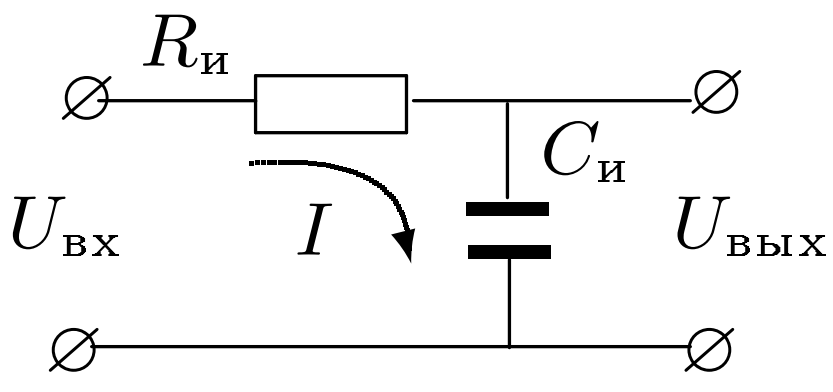
\includegraphics[width=6cm]{RC.png}
    \caption{Интегрирующая ячейка - RC-цепочка}
    \label{rc} %% метка рисунка для ссылки на него
    \end{center}
\end{figure}

Формула (4) тем ближе с истине, чем больше постоянная времени $\tau = RC$ превосходит время процесса. Для  синусоидальных напряжений

\begin{equation}
    U_{вых} = \frac{U_{вх}}{RC\varOmega}, \label{eq:ref}
\end{equation}
где $\varOmega$ - частота сигнала. Зная параметры интегрирующей цепочки, выразим $B$.

\begin{equation}
    |B| = \frac{1}{SN_и} \int U_{вх}dt = \frac{R_иC_и}{SN_и}U_{вых}, \label{eq:ref}
\end{equation}

\section{Экспериментальная установка}
Схема установки изображена на рис. \ref{scheme}. Напряжение сети ($220 B, 50 Гц$) с помощью регулировочного автотрансформатора Ат через разделительный понжающий трансформатор Тр пожается на намагниченную обмотку $N_0$ исследуемого образца. 
Действуещее значение переменного тока в обмотке $N_0$ измеряется амперметром А. Последовательно  с амперметром включено сопротивление $R_0$, напряжение с которого подается на вхд $X$ электронного осциллографа. 

\hyphenation{}
Для измерения магнитной индукции $B$ с измерительной обмотки $N_и$ на вход $RC$-цепочки подается напряжение $U_и(U_{вх})$, пропорциональное согласно (6) производной 
$\dot{B}$, а с интегрирующей ёмкости $C_и$ снимается напряжение $U_C(U_{вых})$, пропорциональное величине $B$, и подаётся на вход $Y$ осциллографа. 

\begin{figure}[H]
    \begin{center}
    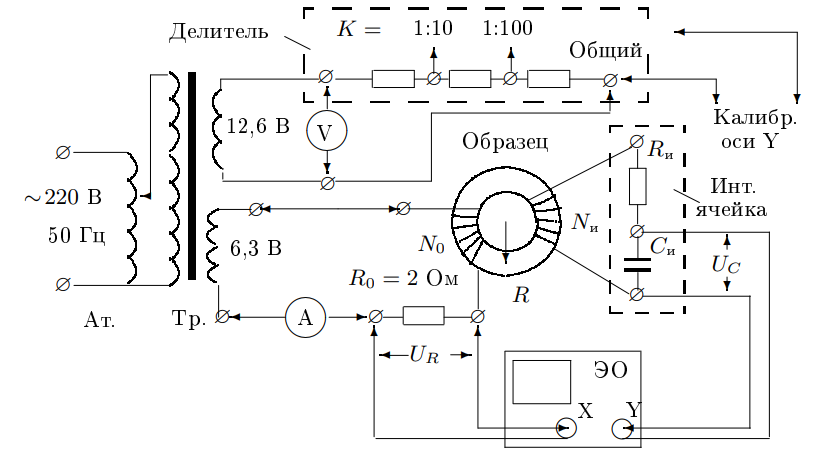
\includegraphics[width=10cm]{scheme.png}
    \caption{Схема установки для исследования и намагничивания образцов}
    \label{scheme} %% метка рисунка для ссылки на него
    \end{center}
\end{figure}

Замкутая кривая, возникающая на экране, воспроизводит петлю гистерезиса. Но чтобы придать этой кривой количественный смысл, необходимо установить
масшатбы изображения (привести калибровку каналов $X$ и $Y$ ЭО).

\textbf{Измерение напряжения с помощью осциллографа}.
Исследуемый сигнал подается на вход $X$. 
Удвоенная амплитуда напряжения характеризуется уравнением: $2U_{x,0}=2xK_x$, x - отклонение от нуля, а $K_x$ -чувствительность усилителя в В/дел.

\textbf{Калибровка горизонтальной оси ЭО} проводится при закороченной обмотке $N_0$, тк эт обмотка с помещенным в нее ферромагнитным образцомне является нелинейным элементом. Амперметр измеряет $I_{эфф}$, текущий через $R_0$.
Тогда измерив длину горизонтальной прямой на экране ЭО, можно рассчитать чувствительность:
\begin{equation}
    m_x = \frac{2R_0\sqrt{2}I_{эфф}}{2x} \frac{B}{дел}, \label{eq:ref}
\end{equation}

\textbf{Калибровка вертикольной оси} проводится с помощью сигнала,м снимаемого чере зделитель напряжения обмотки 12,6$B$ понижающего трасформатора. Вольтметр $V$ измеряет напряжение $U_{эфф}$ на обмотке. Часть этого напряжения снимается 
сделителя с коэффициентом деления $K$ и подается на вход $Y$ ЭО.
Тогда измерив длину вертикальной прямой на экране ЭО, можно рассчитать чувствительность:
\begin{equation}
    m_y = \frac{2\sqrt{2}KU_{эфф}}{2y} \frac{B}{дел}, \label{eq:ref}
\end{equation}
Здесь тероид должен быть отключен, так как несинусоидальный ток нагрузки в первичной обмотке $N_0$ приводит к искажению формы кривой напряжения на обмотке трансформатора, питающий делитель.
Калибровку осей можно использовать для построения кривой гистерезиса в координатах $B$ и $H$. $H$ - рассчитываем из теоремы о циркуляции, $H$ - из формулы (6). 

\textbf{Постоянную времени $RC$-цепочки} можно определить экспериментально. С обмотки 6,3 $B$ на вход интегрирующей цепочки подается синусоидальное напряжение $U_{вх}$. На вход $Y$ поочередно подают $U_{вх}$ и $U_{вых = U_c}$ $RC$-цепочки. 
Тогда можно рассчитать постоянную времени:

\begin{equation}
    \tau = RC = \frac{U_{вх}}{\varOmega U_{вых}}, \label{eq:ref}
\end{equation}

\section{Ход работы}

\begin{enumerate}
    \item Для 3-х образцов (феррит, пермалой, кремистое железо) при помощи ЭО изучаем крайние точки петель гистерезиса. Предельную петлю определяем по появлению "усов", затем, уменьшая ток, снимаем напряжения на подающем и интегрирующих контурах, сответствующие вершинам петель.
    Данные приведены в таблице 

    \begin{table}[H]
        \centering
        \begin{center}
        \end{center}
        \vspace{0.1cm}
        \label{tab:my_label}
        \begin{tabular}{ |p{2cm}|p{2cm}|p{2cm}|p{2cm}|p{2cm}|p{2cm}|}
     \hline
     Феррит x & Феррит y & Пермаллой х & Пермаллой у & Железо х & Железо у\\
     \hline
        44 & 42 & 72 & 90 & 220 & 56\\
     \hline
        40 & 40 & 56 & 90 & 200 & 50\\
       \hline
        35 & 38 & 40 & 70 & 190 & 49\\
       \hline
        32 & 36 & 38 & 60 & 180 & 48\\
       \hline
        28 & 34 & 36 & 54 & 160 & 44\\
        \hline
        24 & 33 & 36 & 46 & 150 & 42\\
       \hline
        20 & 30 & 33 & 28 & 130 & 40\\
       \hline
        18 & 28 & 30 & 16 & 110 & 36\\
        \hline
        12 & 23 & 28 & 11 & 105 & 34\\
        \hline
        10 & 20 & 26 & 7.5 & 90 & 30\\
        \hline
        7 & 14 & 20 & 5 & 86 & 28\\
        \hline
        7 & 10 & 12.5 & 2 & 76 & 25\\
        \hline
        7 & 9 & 5 & 1 & 70 & 22\\
        \hline
        5 & 5 & 0 & 0 & 60 & 17.5\\
        \hline
        3 & 3 & & & 52 & 16\\
        \hline
        1 & 1 & & & 50 & 14\\
        \hline
        0 & 0 & & & 45 & 11\\
        \hline
         & & & & 36 & 9\\
         \hline
         & & & & 32 & 6\\
         \hline
         & & & & 28 & 5\\
         \hline
         & & & & 20 & 2.5\\
         \hline
         & & & & 10 & 0.5\\
         \hline
         & & & & 0 & 0\\
    \hline
    \end{tabular}
    \caption{Обработка данных с образцов}
    \end{table}
    
    Из этих данных рассчитаем $H$, $B$ и построим график зависимости $B(H)$ для образцов, которая будет представлять собой кривую намагничивания.

    \begin{figure}[H]
        \begin{center}
        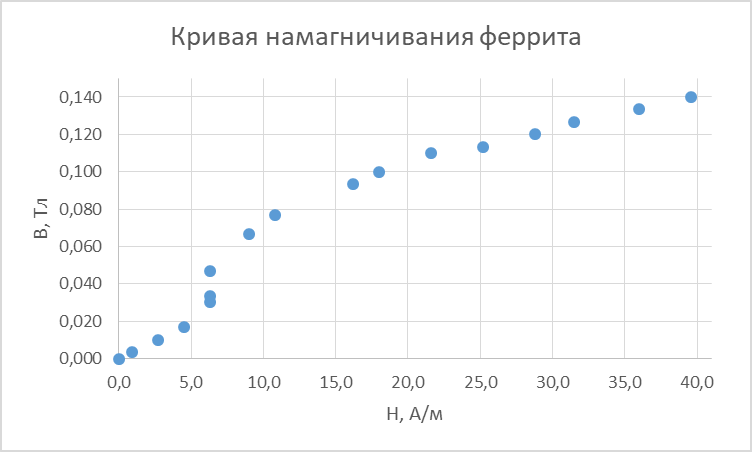
\includegraphics[width=10cm]{ferrit.png}
        \caption{Кривая намагничивания феррита}
        \label{ferrit} 
        \end{center}
    \end{figure}

    \begin{figure}[H]
        \begin{center}
        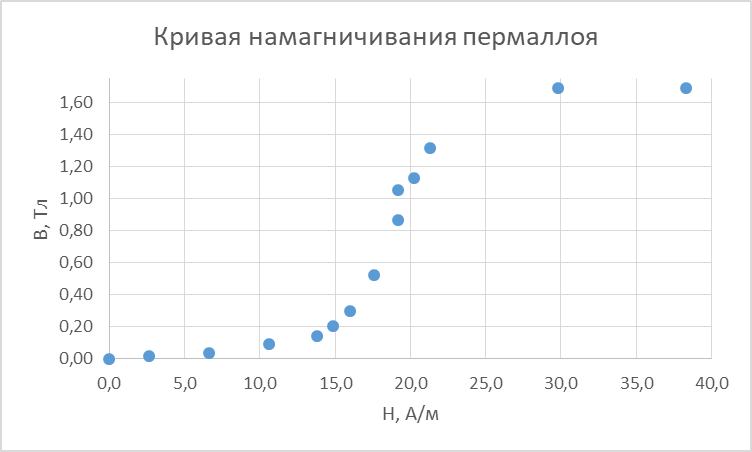
\includegraphics[width=10cm]{pe.png}
        \caption{Кривая намагничивания пермаллоя}
        \label{pe} %% метка рисунка для ссылки на него
        \end{center}
    \end{figure}
    
    \begin{figure}[H]
        \begin{center}
            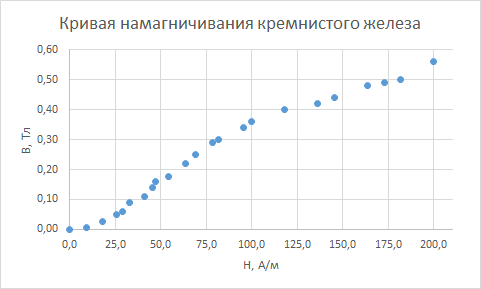
\includegraphics[width=10cm]{fe.PNG}
            \caption{Кривая намагничивания железа}
            \label{fe} %% метка рисунка для ссылки на него
        \end{center}
    \end{figure}
    
    \item Для каждого образца выберем ряд точек, с помощью оценим максимальновозможный коэффициент наклона $\frac{dB}{dH}$ в области насыщения и начальногонамагничивания.
    Зная значения наклона прямой гистерезиса и магнотной постоянной, можно найти значения магнитной проницаемости материалов:

    \begin{equation}
        \mu = \frac{1}{\mu_0}\frac{dB}{dH}, \label{eq:ref}
    \end{equation}   
    где $\mu_0 = 1,26 \cdot 10^{-6} $.

    \begin{figure}[H]
        \begin{center}
            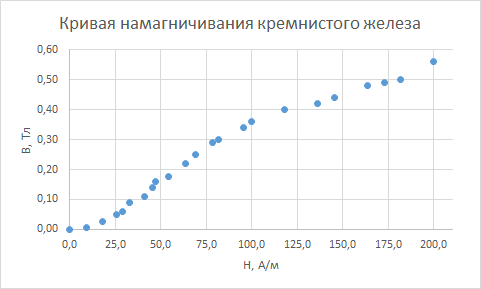
\includegraphics[width=10cm]{fe.PNG}
            \caption{Кривая намагничивания железа}
            \label{fe} %% метка рисунка для ссылки на него
        \end{center}
    \end{figure}

    \begin{figure}[H]
        \begin{center}
            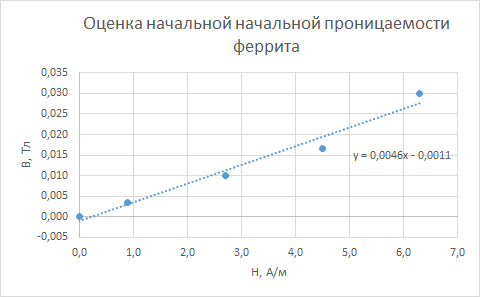
\includegraphics[width=10cm]{проницаемость_феррита_начало.PNG}
            \caption{Оценка магнитной проницаемости феррита}
            \label{fe} %% метка рисунка для ссылки на него
        \end{center}
    \end{figure}

    \begin{figure}[H]
        \begin{center}
            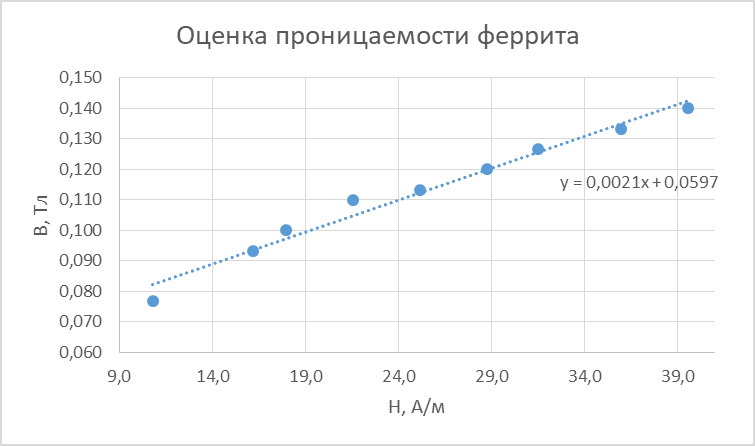
\includegraphics[width=10cm]{проницаемость_феррита_конец.PNG}
            \caption{Оценка магнитной проницаемости феррита}
            \label{fe} %% метка рисунка для ссылки на него
        \end{center}
    \end{figure}

    \begin{figure}[H]
        \begin{center}
            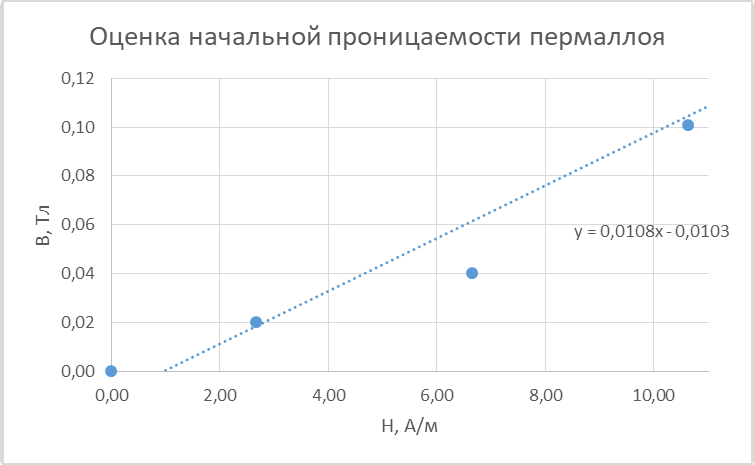
\includegraphics[width=10cm]{проницаемость_пермаллоя_начало.PNG}
            \caption{Оценка магнитной проницаемости пермаллоя}
            \label{fe} %% метка рисунка для ссылки на него
        \end{center}
    \end{figure}

    \begin{figure}[H]
        \begin{center}
            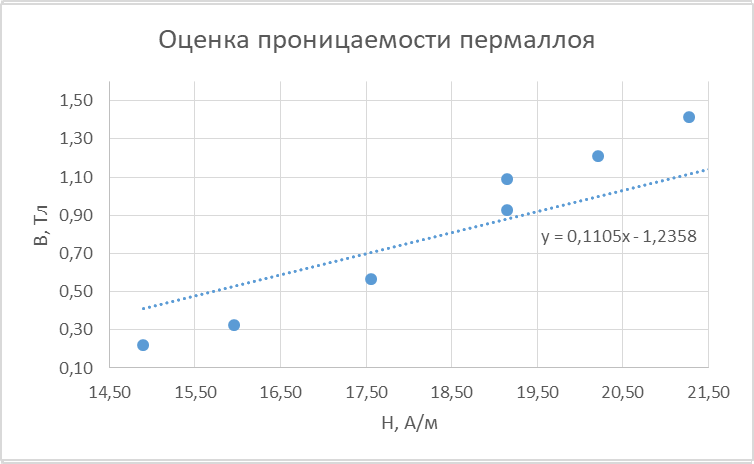
\includegraphics[width=10cm]{проницаемость_пермаллоя_конец.PNG}
            \caption{Оценка магнитной проницаемости пермаллоя}
            \label{fe} %% метка рисунка для ссылки на него
        \end{center}
    \end{figure}

    \begin{figure}[H]
        \begin{center}
            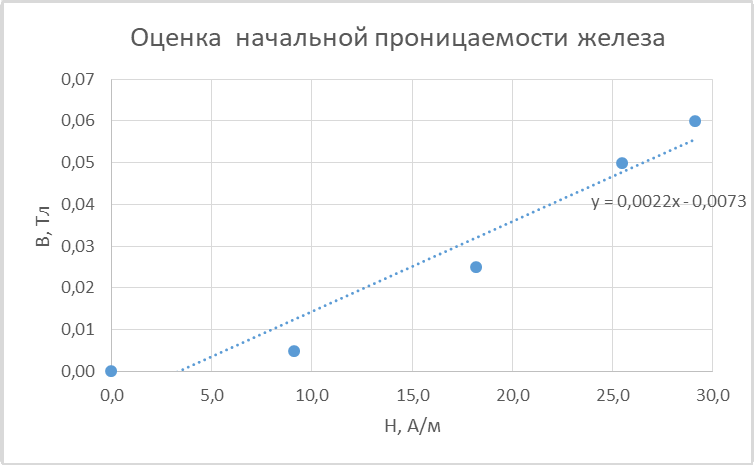
\includegraphics[width=10cm]{проницаемость_железа_начало.PNG}
            \caption{Оценка магнитной проницаемости железа}
            \label{fe} %% метка рисунка для ссылки на него
        \end{center}
    \end{figure}

    \begin{figure}[H]
        \begin{center}
            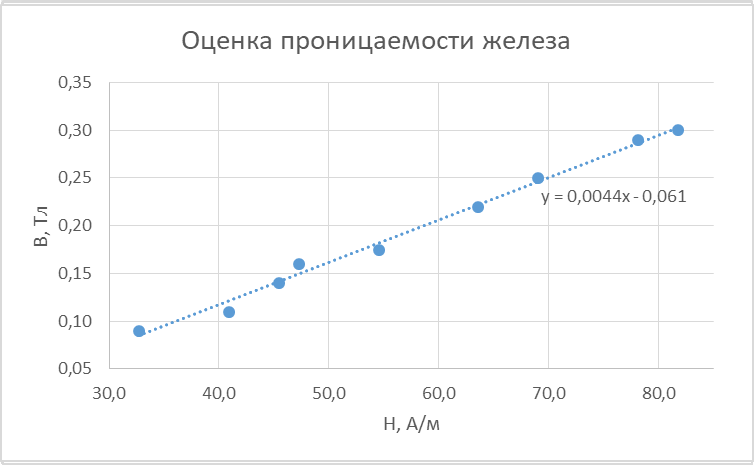
\includegraphics[width=10cm]{проницаемость_железа_конец.PNG}
            \caption{Оценка магнитной проницаемости железа}
            \label{fe} %% метка рисунка для ссылки на него
        \end{center}
    \end{figure}
    
\item Рассмотрим петлю гистерезиса в предельном положении. Координата предельной точки оси $x$ будет соответствовать коэрцитивной силе $H_c$, а по оси $y$ - индукции насыщения $B_s$.

\begin{equation}
    H = \frac{IN_0}{2\pi R}
\end{equation}
\begin{equation}
    B = \frac{R_иC_и}{SN}U_y
\end{equation}
Занесем эти данные также в таблицу.

\begin{table}[H]
    \centering
    \begin{center}
    \end{center}
    \vspace{0.1cm}
    \label{tab:my_label}
    \begin{tabular}{ |p{2cm}|p{1.5cm}|p{3cm}|p{1.5cm}|p{2cm}|p{1cm}|p{1.3cm}|}
 \hline
 Образец & $k\cdot10^{-3}$ & $\mu_{max}\cdot10^{3} Гн/м$ & $k\cdot10^{-3}$ & $\mu\cdot10^{3} Гн/м$ & $B_c Тл$ & $H_c А/м$ \\
 \hline
    Феррит & 4.6 & 3.65 & 2.1 & 1.6 & 0.14 & 7.2\\
 \hline
    Пермаллой & 110.5 & 87.7 & 10.8 & 8.6 & 1.8& 25.5\\
   \hline
    Кремнистое железо & 4.4 & 3.5 & 2.2 & 1.7 & 0.6 & 54.6\\
\hline
\end{tabular}
\caption{Обработка данных с образцов}
\end{table}

\item Рассчитаем чувствительности по осям. Начнем с канала $X$. 

\begin{equation}
    m_x = \frac{2R_0\sqrt{2}I_{эфф}}{2x} = 19 мB
\end{equation}   
Здесь $R_0 = 0.2 Ом$, $I_{эфф} = 0.273 А$, $2x = 8$. На ЭО  чувствительность $K_x = 20 мВ$. Тогда $\Delta m_x / m_x = 5\% $ 
\\ Чувствительность канала $Y$:

\begin{equation}
    m_y = \frac{2\sqrt{2}KU_{эфф}}{2y} = 49 мВ
\end{equation}
Здесь $U_{эфф} = 135 мВ$, $2y = 7.8$. Тогда $\Delta m_y / m_y = 2\% $ 

\item Рассчитаем постоянную времени.

\begin{equation}
    \tau = \frac{U_{вх}}{\varOmega U_{вых} = 0.38 c}
\end{equation}

Здесь $U_{вх} = 600 мВ$, $U_{вых} = 5 мВ$, $\varOmega = 2 \pi \cdot 50 Гц$.

Cравним с рассчетами по формуле $\tau = RC = 0.4 c$. \\
Здесь $R = 20 кOм$, $C = 20 мкФ$. Тогда $\Delta \tau / \tau = 5\%$

\end{enumerate}

\section{Вывод}

Сравним полученные значения с табличными.

\begin{table}[H]
    \centering
    \begin{center}
    \end{center}
    \vspace{0.1cm}
    \label{tab:my_label}
    \begin{tabular}{|p{4cm}|p{2.5cm}|p{2cm}|p{2cm}|p{2cm}|}
 \hline
 Образец & $\mu_{max}, 10^3Гн/м$ & $\mu, 10^3Гн/м$ & $B_c, Тл$ & $H_c, А/м$ \\
 \hline
    Феррит & 3.65 & 1.6 & 0.14 & 7.2\\
 \hline
    Пермаллой & 87.7 & 8.6 & 1.8& 25.5\\
   \hline
    Кремнистое железо & 3.5  & 1.7 & 0.6 & 54.6\\
    \hline
    Феррит, табл &  & 0.01 - 20 & 0.1 - 0.4 & 4 - 1600\\
 \hline
    Пермаллой, табл & 100 & 4 & 1.05 & 4\\
   \hline
    Кремнистое железо, табл & 7 & 0.5 & 2 & 12\\
\hline
\end{tabular}
\caption{Сравнительная таблица}
\end{table}

Как видно из таблицы, характерные максимальные и начальные значения магнитной проницаемости согласуются с табличными. Для $B_c$ и $H_c$ совпадение наблюдается только для образца феррита. Значение  индукции других образцов близки по порядку, а вот коэрцитивной силы разнятся. Итоговые различия можно связать с неточным получением предельных петель, расплывчатостью картинки.\\ 

В ходе лабораторной работы
\begin{enumerate}
    \item Изучили явление петли гистерезиса на примере трех тороидальных образцов из различных ферромагнетиков.
    \item Получили оценки максимальных значений магнитной проницаемости материалов.
    \item Получили значения коэрцитивной силы и индукции насыщения.
\end{enumerate}


\newpage





\end{document}